% !TEX root = main.tex

%%%-------------------------------------------
\section*{Листочек 6: свёрточные сети} 

\addcontentsline{toc}{section}{Листочек 6: свёрточные сети}

\epigraph{Урра! Отлично сработано, ребятки. Давайте завтра не придем? Возьмем отгул на денек? Вы пробовали шаурму? В двух кварталах отсюда делают какую-то шаурму. Не знаю, что это, но мне хочется.}{\textit{Тони Старк (Мстители, 2012)}}

% Нарезать на задачи: 
% https://arxiv.org/pdf/1603.07285.pdf

\begin{problem}{(Свёртка своими руками)}
У Маши есть картинка и свёртка, которую она хочет применить к этой картинке.
    \begin{figure}[H]
    \begin{minipage}{0.49\linewidth} 
        \centering
        \begin{tikzpicture}[scale=.8,every node/.style={minimum size=1cm}, on grid]
                \draw[fill=green,opacity=0.4] (0,-2) rectangle (5,3);
                \draw[draw=green,thick] (0,-2) grid (5,3);
                \node (00) at (0.5,2.5) {3};
                \node (01) at (1.5,2.5) {3};
                \node (02) at (2.5,2.5) {2};
                \node (03) at (3.5,2.5) {1};
                \node (04) at (4.5,2.5) {0};
                
                \node (10) at (0.5,1.5) {0};
                \node (11) at (1.5,1.5) {0};
                \node (12) at (2.5,1.5) {1};
                \node (13) at (3.5,1.5) {3};
                \node (14) at (4.5,1.5) {1};
                
                \node (20) at (0.5,0.5) {3};
                \node (21) at (1.5,0.5) {1};
                \node (22) at (2.5,0.5) {2};
                \node (23) at (3.5,0.5) {2};
                \node (24) at (4.5,0.5) {3};
                
                \node (30) at (0.5,-0.5) {3};
                \node (31) at (1.5,-0.5) {1};
                \node (32) at (2.5,-0.5) {2};
                \node (33) at (3.5,-0.5) {2};
                \node (34) at (4.5,-0.5) {3};
                
                \node (40) at (0.5,-1.5) {3};
                \node (41) at (1.5,-1.5) {1};
                \node (42) at (2.5,-1.5) {2};
                \node (43) at (3.5,-1.5) {2};
                \node (44) at (4.5,-1.5) {3};
        \end{tikzpicture}
        \\ Картинка Маши
    \end{minipage} 
    \hfill
    \begin{minipage}{0.49\linewidth} 
        \centering
        \begin{tikzpicture}[scale=.8,every node/.style={minimum size=1cm}, on grid]
                \draw[fill=blue,opacity=0.4] (0,0) rectangle (3,3);
                \draw[draw=blue,thick] (0,0) grid (3,3);
                \node (00) at (0.5,2.5) {0};
                \node (01) at (1.5,2.5) {1};
                \node (02) at (2.5,2.5) {2};
                \node (10) at (0.5,1.5) {2};
                \node (11) at (1.5,1.5) {2};
                \node (12) at (2.5,1.5) {0};
                \node (20) at (0.5,0.5) {0};
                \node (21) at (1.5,0.5) {1};
                \node (22) at (2.5,0.5) {2};
        \end{tikzpicture}
        \\ Свёртка Маши
    \end{minipage} 
    \end{figure}
    \begin{enumerate} 
        \item Сделайте свёртку картинки без сдвигов и дополнений. К тому, что получилось применить max pooling и average pooling размера $2 \times 2$.
        \item Примените к исходной картинке свёртку с параметром сдвига (stride) равным $2$.
        \item Примените к исходной картинке свёртку с параметром сдвига (stride) равным $3$.
        \item Примените к исходной картинке свёртку с дополнением нулями (zero padding) и параметром сдвига (stride) равным $0$.
    \end{enumerate} 
\end{problem}


\begin{problem}{(Ядра)}
У Маши есть куча ядер для свёрток. Догадайтесь какое из них что делает:

    \begin{minipage}{0.18\linewidth} 
        \centering
        \begin{tikzpicture}[scale=.8,every node/.style={minimum size=1cm}, on grid]
                \draw[fill=blue,opacity=0.4] (0,0) rectangle (3,3);
                \draw[draw=blue,thick] (0,0) grid (3,3);
                \node (00) at (0.5,2.5) {0};
                \node (01) at (1.5,2.5) {0};
                \node (02) at (2.5,2.5) {0};
                \node (10) at (0.5,1.5) {0};
                \node (11) at (1.5,1.5) {1};
                \node (12) at (2.5,1.5) {0};
                \node (20) at (0.5,0.5) {0};
                \node (21) at (1.5,0.5) {0};
                \node (22) at (2.5,0.5) {0};
        \end{tikzpicture}
    \end{minipage} 
    \hfill
    \begin{minipage}{0.18\linewidth} 
        \centering
        \begin{tikzpicture}[scale=.8,every node/.style={minimum size=1cm}, on grid]
                \draw[fill=blue,opacity=0.4] (0,0) rectangle (3,3);
                \draw[draw=blue,thick] (0,0) grid (3,3);
                \node (00) at (0.5,2.5) {-1};
                \node (01) at (1.5,2.5) {-1};
                \node (02) at (2.5,2.5) {-1};
                \node (10) at (0.5,1.5) {-1};
                \node (11) at (1.5,1.5) {8};
                \node (12) at (2.5,1.5) {-1};
                \node (20) at (0.5,0.5) {-1};
                \node (21) at (1.5,0.5) {-1};
                \node (22) at (2.5,0.5) {-1};
        \end{tikzpicture}
    \end{minipage} 
    \hfill
    \begin{minipage}{0.18\linewidth} 
        \centering
        \begin{tikzpicture}[scale=.8,every node/.style={minimum size=1cm}, on grid]
                \draw[fill=blue,opacity=0.4] (0,0) rectangle (3,3);
                \draw[draw=blue,thick] (0,0) grid (3,3);
                \node (00) at (0.5,2.5) {-1};
                \node (01) at (1.5,2.5) {-1};
                \node (02) at (2.5,2.5) {-1};
                \node (10) at (0.5,1.5) {-1};
                \node (11) at (1.5,1.5) {8};
                \node (12) at (2.5,1.5) {-1};
                \node (20) at (0.5,0.5) {-1};
                \node (21) at (1.5,0.5) {-1};
                \node (22) at (2.5,0.5) {-1};
        \end{tikzpicture}
    \end{minipage} 
    \hfill
    \begin{minipage}{0.18\linewidth} 
        \centering
        \begin{tikzpicture}[scale=.8,every node/.style={minimum size=1cm}, on grid]
                \draw[fill=blue,opacity=0.4] (0,0) rectangle (3,3);
                \draw[draw=blue,thick] (0,0) grid (3,3);
                \node (00) at (0.5,2.5) {-1};
                \node (01) at (1.5,2.5) {-1};
                \node (02) at (2.5,2.5) {-1};
                \node (10) at (0.5,1.5) {-1};
                \node (11) at (1.5,1.5) {8};
                \node (12) at (2.5,1.5) {-1};
                \node (20) at (0.5,0.5) {-1};
                \node (21) at (1.5,0.5) {-1};
                \node (22) at (2.5,0.5) {-1};
        \end{tikzpicture}
    \end{minipage} 
    \hfill
    \begin{minipage}{0.18\linewidth} 
        \centering
        \begin{tikzpicture}[scale=.8,every node/.style={minimum size=1cm}, on grid]
                \draw[fill=blue,opacity=0.4] (0,0) rectangle (3,3);
                \draw[draw=blue,thick] (0,0) grid (3,3);
                \node (00) at (0.5,2.5) {-1};
                \node (01) at (1.5,2.5) {-1};
                \node (02) at (2.5,2.5) {-1};
                \node (10) at (0.5,1.5) {-1};
                \node (11) at (1.5,1.5) {8};
                \node (12) at (2.5,1.5) {-1};
                \node (20) at (0.5,0.5) {-1};
                \node (21) at (1.5,0.5) {-1};
                \node (22) at (2.5,0.5) {-1};
        \end{tikzpicture}
    \end{minipage} 
% - границы
% - повороты
% - сдвиги 
\end{problem}

\newpage

\begin{problem}{(Крестики и нолики)}
Маша хочет научить компьютер играть в крестики и нолики. На первом шаге ей надо научить алгоритм распознавать есть ли крестик на картинке. Под ноликом понимается любая фигура с дырой в середине. Под крестиком понимается любая фигура из двух пересекающихся линий.

Алгоритм должен быть устроен следующим образом. На первом шаге одна или несколько свёрток проходят по картинке. На втором шаге по результатам свёрток принимается решение. Например, берётся максимальное получившееся число и сравнивается с каким-то порогом. Классификатор крестиков и ноликов должен работать безупречно. Помогите Маше придумать такой классификатор. 

\begin{enumerate} 
    \item  В мире Маши на картинках могут быть нарисованы либо крестики либо нолики. Все картинки, подающиеся на вход алгоритма могут быть только размера $4 \times 4$. Примеры крестиков и ноликов нарисованы ниже. 
    
    \begin{minipage}{0.22\linewidth} 
        \centering
        \begin{tikzpicture}[scale=.8,every node/.style={minimum size=1cm}, on grid]
                \draw[fill=green,opacity=0.4] (0,-1) rectangle (4,3);
                \draw[draw=green,thick] (0,-1) grid (4,3);
                \node (00) at (0.5,2.5) {1};
                \node (01) at (1.5,2.5) {1};
                \node (02) at (2.5,2.5) {1};
                \node (03) at (3.5,2.5) {0};
                
                \node (10) at (0.5,1.5) {1};
                \node (11) at (1.5,1.5) {0};
                \node (12) at (2.5,1.5) {1};
                \node (13) at (3.5,1.5) {0};
                
                \node (20) at (0.5,0.5) {1};
                \node (21) at (1.5,0.5) {0};
                \node (22) at (2.5,0.5) {1};
                \node (23) at (3.5,0.5) {0};
                
                \node (30) at (0.5,-0.5) {1};
                \node (31) at (1.5,-0.5) {1};
                \node (32) at (2.5,-0.5) {1};
                \node (33) at (3.5,-0.5) {0};
        \end{tikzpicture}
        \\ нолик
    \end{minipage} 
    \hfill
    \begin{minipage}{0.22\linewidth} 
        \centering
        \begin{tikzpicture}[scale=.8,every node/.style={minimum size=1cm}, on grid]
                \draw[fill=green,opacity=0.4] (0,-1) rectangle (4,3);
                \draw[draw=green,thick] (0,-1) grid (4,3);
                \node (00) at (0.5,2.5) {0};
                \node (01) at (1.5,2.5) {0};
                \node (02) at (2.5,2.5) {1};
                \node (03) at (3.5,2.5) {0};
                
                \node (10) at (0.5,1.5) {0};
                \node (11) at (1.5,1.5) {1};
                \node (12) at (2.5,1.5) {0};
                \node (13) at (3.5,1.5) {1};
                
                \node (20) at (0.5,0.5) {0};
                \node (21) at (1.5,0.5) {0};
                \node (22) at (2.5,0.5) {1};
                \node (23) at (3.5,0.5) {0};
                
                \node (30) at (0.5,-0.5) {0};
                \node (31) at (1.5,-0.5) {0};
                \node (32) at (2.5,-0.5) {0};
                \node (33) at (3.5,-0.5) {0};
        \end{tikzpicture}
        \\ нолик
    \end{minipage} 
    \hfill
    \begin{minipage}{0.22\linewidth} 
        \centering
        \begin{tikzpicture}[scale=.8,every node/.style={minimum size=1cm}, on grid]
                \draw[fill=green,opacity=0.4] (0,-1) rectangle (4,3);
                \draw[draw=green,thick] (0,-1) grid (4,3);
                \node (00) at (0.5,2.5) {0};
                \node (01) at (1.5,2.5) {1};
                \node (02) at (2.5,2.5) {0};
                \node (03) at (3.5,2.5) {1};
                
                \node (10) at (0.5,1.5) {0};
                \node (11) at (1.5,1.5) {0};
                \node (12) at (2.5,1.5) {1};
                \node (13) at (3.5,1.5) {0};
                
                \node (20) at (0.5,0.5) {0};
                \node (21) at (1.5,0.5) {1};
                \node (22) at (2.5,0.5) {0};
                \node (23) at (3.5,0.5) {1};
                
                \node (30) at (0.5,-0.5) {0};
                \node (31) at (1.5,-0.5) {0};
                \node (32) at (2.5,-0.5) {0};
                \node (33) at (3.5,-0.5) {0};
        \end{tikzpicture}
        \\ крестик 
    \end{minipage} 
    \hfill
    \begin{minipage}{0.22\linewidth} 
        \centering
        \begin{tikzpicture}[scale=.8,every node/.style={minimum size=1cm}, on grid]
                \draw[fill=green,opacity=0.4] (0,-1) rectangle (4,3);
                \draw[draw=green,thick] (0,-1) grid (4,3);
                \node (00) at (0.5,2.5) {0};
                \node (01) at (1.5,2.5) {1};
                \node (02) at (2.5,2.5) {0};
                \node (03) at (3.5,2.5) {0};
                
                \node (10) at (0.5,1.5) {1};
                \node (11) at (1.5,1.5) {1};
                \node (12) at (2.5,1.5) {1};
                \node (13) at (3.5,1.5) {1};
                
                \node (20) at (0.5,0.5) {0};
                \node (21) at (1.5,0.5) {1};
                \node (22) at (2.5,0.5) {0};
                \node (23) at (3.5,0.5) {0};
                
                \node (30) at (0.5,-0.5) {0};
                \node (31) at (1.5,-0.5) {1};
                \node (32) at (2.5,-0.5) {0};
                \node (33) at (3.5,-0.5) {0};
        \end{tikzpicture}
        \\ крестик 
    \end{minipage}
    
    \item  Предположим, что теперь кроме крестиков и ноликов в нашем мире существуют ещё и другие любые картинки. Как можно модернизировать ваш алгоритм, чтобы он по-прежнему стабильно работал с безупречным качеством? 
\end{enumerate} 
\end{problem}

\begin{problem}{(Свёрточный и полносвязный)}
Маше рассказали, что свёрточный слой --- это полносвязный слой с некоторыми ограничениями. Она хочет разобраться, что это за ограничения. На вход в слой идёт чёрно-белое изображение размера $4 \times 4.$ Каждый пиксель изображения --- отдельная переменная.
    \begin{enumerate} 
        \item Нарисуйте с помощью кругляшей и стрелочек полносвязным слой, который обрабатывает картинку. Подпишите все веса. Нарисуйте свёрточный слой в таком же формате. На картинке часть связей исчезнет, а часть весов станет одинаковой. 
    
        \item Запишите свёрточный слой с помощью перемножения матриц в виде $H = X \cdot W.$ Как выглядит матрица $W$? Как через свёрточный слой можно сделать шаг обратного распространения ошибки? 
    \end{enumerate} 
\end{problem}


\begin{problem}{(Число параметров)}
На вход в нейронную сетку идёт изображение рукописной цифры размера $28 \times 28$.
\begin{enumerate}
    \item Маша вытягивает изображение в длинный вектор и использует полносвязную сетку для классификации изображений. В сетке идёт один полносвязный слой из $1000$ нейронов. После идёт слой, который осуществляет классификацию изображения на $10$ классов. Сколько параметров нужно оценить?
    
    \item \label{lanet} Маша вместо полносвязной сетки использует свёрточную. На первом шаге делается $6$ свёрток размера $5 \times 5$. На втором шаге делается max-pooling размера $2 \times 2$. На третьем $16$ свёрток размера $5\times 5$. На четвёртом max-pooling размера $2 \times 2$. На пятом картинка вытягивается в длинный вектор. Далее идут три полносвязных слоя размеров $120, 84, 10$. В конце делается softmax. После каждой свёртки и полносвязного слоя, кроме последнего, в качестве функции активации используется $ReLU.$ 
    
    \begin{center}    
    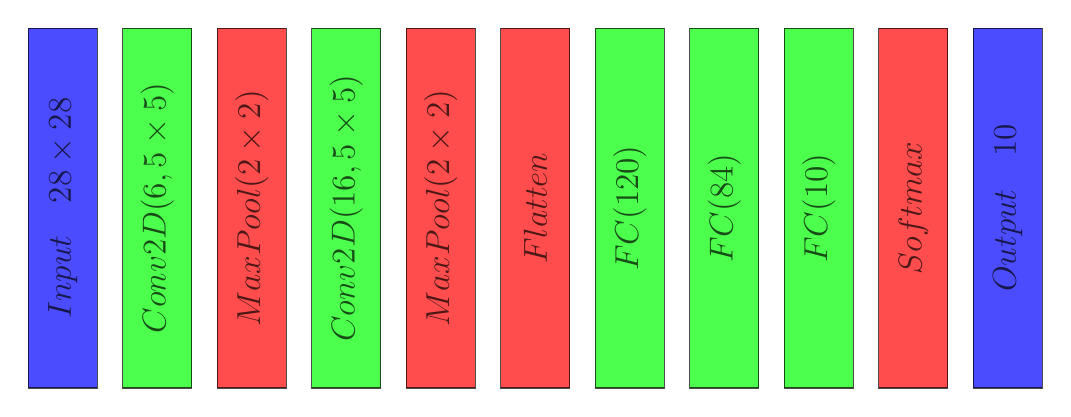
\begin{tikzpicture}[scale=.8]
    \tikzstyle{st}=[draw=black, opacity=0.7, minimum height=25pt,minimum width=130pt,inner sep=2pt,rotate=90];
    
	\node at (0, 0) [st, fill=blue] { \large $Input \quad 28 \times 28$};
	\node at (1.5, 0) [st, fill=green] { \large $Conv2D(6, 5 \times 5)$};
	\node at (3, 0) [st, fill=red] { \large $MaxPool(2\times2)$};
	\node at (4.5, 0) [st, fill=green] { \large $Conv2D(16, 5 \times 5)$};
	\node at (6, 0) [st, fill=red] { \large $MaxPool(2\times2)$};
	\node at (7.5, 0) [st, fill=red] { \large $Flatten$};
	\node at (9, 0) [st, fill=green] { \large $FC(120)$};
	\node at (10.5, 0) [st, fill=green] { \large $FC(84)$};
	\node at (12, 0) [st, fill=green] { \large $FC(10)$};
	\node at (13.5, 0) [st, fill=red] { \large $Softmax$};
	\node at (15, 0) [st, fill=blue] { \large $Output \quad 10$};
    \end{tikzpicture}
    \end{center} 
    
    Сколько параметров необходимо будет оценить в такой модели? Какого размера будут выходы из каждого слоя? 
    
    \item Маша использует архитектуру из пункта \ref{lanet}, но все свёртки делает с дополнением нулями (zero padding). Как изменится число оцениваемых параметров? Какого размера будут выходы из каждого слоя? 
    
    \item Маша использует архитектуру из пункта \ref{lanet}, но все свёртки делает с дополнением нулями (zero padding) и параметром сдвига (stride) равным $2$. ак изменится число оцениваемых параметров? Какого размера будут выходы из каждого слоя?
\end{enumerate}
\end{problem}

% \begin{sol}
% У нас $28^2 = 784$ входа. Весов между входным и полносвязным слоями будет 
% \[ (784 + 1)\cdot 1000 = 785000.\] 
% Единица отвечает за константу для каждого из $1000$ нейронов. Между полносвязным и итоговым слоем
% \[(1000 + 1) \cdot 10 = 10010. \]
% \end{sol} 


\begin{problem}{(Поле обзора)}
    Маша хочет найти котика размера $512 \times 512$ пикселей. Для этого она использует свёртки размера $5 \times 5$ без дополнения нулями (zero padding) После каждого свёрточного слоя Маша делает max-pooling.
    \begin{enumerate}
        \item Через сколько слоёв поле восприятия Машиной нейросетки впервые охватит котейку?
        
        \item Маша хочет поменять max-pooling на свёртки со сдвигом (stride) так, чтобы котейка находился за такое же число слоёв. Какой размер сдвига ей надо выбрать? 
        
        \item Пусть $s$ --- величина сдвига, $k$ --- размер свёртки, $m$ --- размер пулинга, $n$ --- номер слоя. Выпишите формулу, по которой можно найти размер поля видимости (receptive field). % (2n + 1) \times (2n + 1)
    \end{enumerate}
    % Нарезать на задачи: https://distill.pub/2019/computing-receptive-fields/
\end{problem}


\begin{problem}{(Снова число параметров)}

Маша собирает разные архитектуры. Помогите ей оценить число параметров для каждой из них. 

\begin{enumerate} 
    \item У Маши есть свёрточный слой. На вход в свёрточный слой идёт изображение с $C_{in}$ каналами размера $W \times H$. Маша использует $C_{out}$ фильтров размера $W_k \cdot H_k$. Сколько параметров ей предстоит оценить?
    
    \item 
    
    \item  \todo[inline]{Сюда вариант с подсчётом числа параметров в сепарабельной свёртке}
    
\end{enumerate} 
\end{problem}
% \begin{sol}
% $(W_k \cdot H_k \cdot C_{in} + 1) \cdot C_{out}$
% \end{sol} 


\begin{problem}{(Скользящее среднее)}
Скользящее среднее --- это свёртка, которая работает для вектора. Опишите как именно она работает. Какой физический смысл стоит за размером такой свёртки и дополнением нулями? 
% def moving_average(x, w):
%     return np.convolve(x, np.ones(w), 'valid') / w
\end{problem} 




% \begin{problem}{(Рекур для поля обзора\footnote{По мотивам: \url{https://distill.pub/2019/computing-receptive-fields/})}
%     Пусть у нас есть вектор размера $n$. На нём отрабатывают одномерные свёртки размера $k$ с шагом $s$. Как поле обзора для $i$-го слоя зависит от поля обзора для $i-1$ слоя? Выпишите формулу в явном виде. 
    

%     Пусть у нас есть два свёрточных слоя размера $k \times k$. 
    
%     На подумать: как скип-конкешн и батч-нормализация влияют на поле обзора? 
    
%     Insight: Skip-connections may provide more paths, however, based on [7], they tend to make the effective receptive field smaller.
    
%     During training, batch normalization parameters are computed based on all the channel elements of the feature map. Thus, one can state that its receptive field is the whole input image.
    
    
% \end{problem}
% \begin{sol}
% $r_{i - 1} = s_i \cdot r_i + (k_i - s_i)$


% \end{sol} 

